\newcommand{\repeatcaption}[2]{%
  \renewcommand{\thefigure}{\ref{#1}}%
  \caption{#2 (repeated from page \pageref{#1})}%
}


\chapter{2. Background}

To provide background for BikeBump, this background section considers the challenges of urban planning from a historical stand point looking into these perspectives:
\begin{itemize}
  \item Examining the physicality of democratic decision making, starting
    from ancient Athens to present town meetings in the United States.
  \item Exploring the idea that urban planning connects social issues to physical sites
  \item What kind of issues planners face today. 
  \item Consider technologies that our modern society can leverage and
    explore how those it can support the complicated task of decision
    making. 
\end{itemize}

\section{First traces of direct democracy and the scale of the city}
It is clear that modern smartphone technologies have potential to support a
direct democracy model in social planning. But before discussing these
modern techniques, it is important to consider the underlying mechanism of
how we plan as a crowd.
When thinking about urban designing issues, ``scale'' is a key element
despite the fact the virtual tools have no constraints.
The diagram in Figure \ref{fig:diagram_primitive} is the most primitive
form showing the relationship between the community and the target of urban
planning, infrastructure, and buildings. The border of two environments is
illustrated to be the infrastructure, which is the natural environment and
built environment. We also have the social environment, which is the
community.

\begin{figure}
  
\includegraphics[width=\textwidth]{chapters/2/fig/primitive.png}               
  \caption[layers of environments]{\textfb{The first form of a city and
    layers of environments} We see the community or the society in the middle
    which is the social environment. The social environment is included by the
    `built environment', a physical and artificial region, that was first
    realized in the Athens. The infrastructure functions as the border between
    this artificial region and the rest. The arrow indicates the community
    modifies the infrastructure to meet their own needs. Athens and similar
    polices are considered as communal cities, which the physical and
  artificial environment was planned first before community was allocated.}
  \label{fig:diagram_primitive}
\end{figure}

We see the arrow from the community to modify the infrastructure. This
simplest form does not have any distinction within the community, and the
entire process is lead and examined and executed from the whole.
This form of this democracy is considered to be the very first form
of this kind in ancient Greek. While we may see this as a pure form of
equal political participation, it was limited to men over 18 that had
military practice having the right to speak and vote for each gathering.
Moreover, critics pointed that it was biased by individual member groups
which dominated the proceedings, and unbalanced knowledge levels to make an
informed decisions. It is considered the very first form of direct
democracy and people gathered on the hill of Pnyx as frequent as once in
ten days. The hill of Pnyx had the capacity of 5000 to 13000 people, and
the resolved issues took immediate effect.

As it was primitive in the context of democracy, it was primitive in the
sense of urban planning as well. Before this era, cities spontaneously
emerged by villages and tribes merging and splitting organically. Athens
was one of the first examples that were artificially planned using grids,
coming from the fact it was a colony and the planner Hippodamus (father of
European urban planning) had to allocate residents.
Aside from the gathering and voting at the hill, there were places that men
will meet and supplement information exchange and have political
discussions very close to their daily lives which are a room called the
oikos. This room was adjacent to the courtyard and was open to the public.
Political theorist Hannah Arendt pointed both of this early stage of the
built environment and policy had an intimate relation between each other.
Since the wall separating the oikos and the other rooms was called the
nemein, having a different meaning of distribution, or property, which in
turns has origins to the word nomos, which means law. Thus a physical
structure like a wall had very similar functions as law. 

Lawrence Lessig pointed out in his book "code" that there are four factors
to constrain human behavior; "architecture," "law," "market," "norm."
\cite{lessig2009code} We can see that in the age of the Athens, architecture, and the law was undifferentiated and shared their origin. 

One form of direct democracy that we can observe today is the town meetings
in north east region of the U.S. Massachusetts cities with less than the
population of 6,000 are permitted to open town meetings and decide social
issues. Although the type of problems in consideration will be different
compared to the ancient times, it is similar in the sense that the citizens
pass knowledge and have interaction within another, to collectively
discuss.

\begin{marginfigure}[{-20cm}]
  \includegraphics[width=\textwidth]{chapters/2/fig/town_meeting01.png}               
  \caption[town meetings: moderator]{town meetings}
  \label{fig:town_meeting}
\end{marginfigure}

\begin{marginfigure}[{-10cm}]
  \includegraphics[width=\textwidth]{chapters/2/fig/town_meeting02.png}               
  \caption[town meetings: voting]{standing up for vote}
  \label{fig:spin_margin}
\end{marginfigure}

\marginnote{a town meeting at Warren MA, 2014.11}

It is said that the Roman Republic started this representative
democracy, and the global majority live in this form of democracy
since then. The worlds total population has continued to rise having
more population and density.

The population increase and manual vote counting become too costly to continue a direct democracy method.

\begin{figure}[!htb]
  
\includegraphics[width=\textwidth]{chapters/2/fig/representative.png}               
  \caption[representative democracy]{As cities grew in size and density, it
    was no longer feasible to operate in a direct democracy model, the social
    environment changed its size into a pyramid where planners, governors,
  stakeholders, land owners plan and execute to change the city's infrastructure.}
  \label{fig:diagarm_representative}
\end{figure}

This created a pyramid structure, a top down method that is elected by a
broad community.

\begin{figure}[!htb]
  
\includegraphics[width=\textwidth]{chapters/2/fig/opinion.png}               
  \caption[gathering data from the crowd]{The top part of the pyramid gathers data from the community. This is accomplished in various ways and media technology have been innovated how to do this. Now are able to individually provide opinions to the planners.}
  \label{fig:diagram_opinion}
\end{figure}

Media technology such as the telephones and email, allowed the crowd to
have a communication path to the top. Yet the form of communication is very
different from town meetings, since these media are usually isolated one to
one methods of communications. Urban Planners have invented methods to
collect opinions in a centralized way to effectively collect opinions. We
can categorize these methods based on the amount of information that is
exchanged (\ref{fig:spetrum}}). Smaller the information per transaction,
the easier to process, thus the tool is structured. For example,
polls and surveys are limited in information but are easy to visualize or
even directly interpreted as the collective decision.

% revise this diagram
\begin{figure}[!htb]
  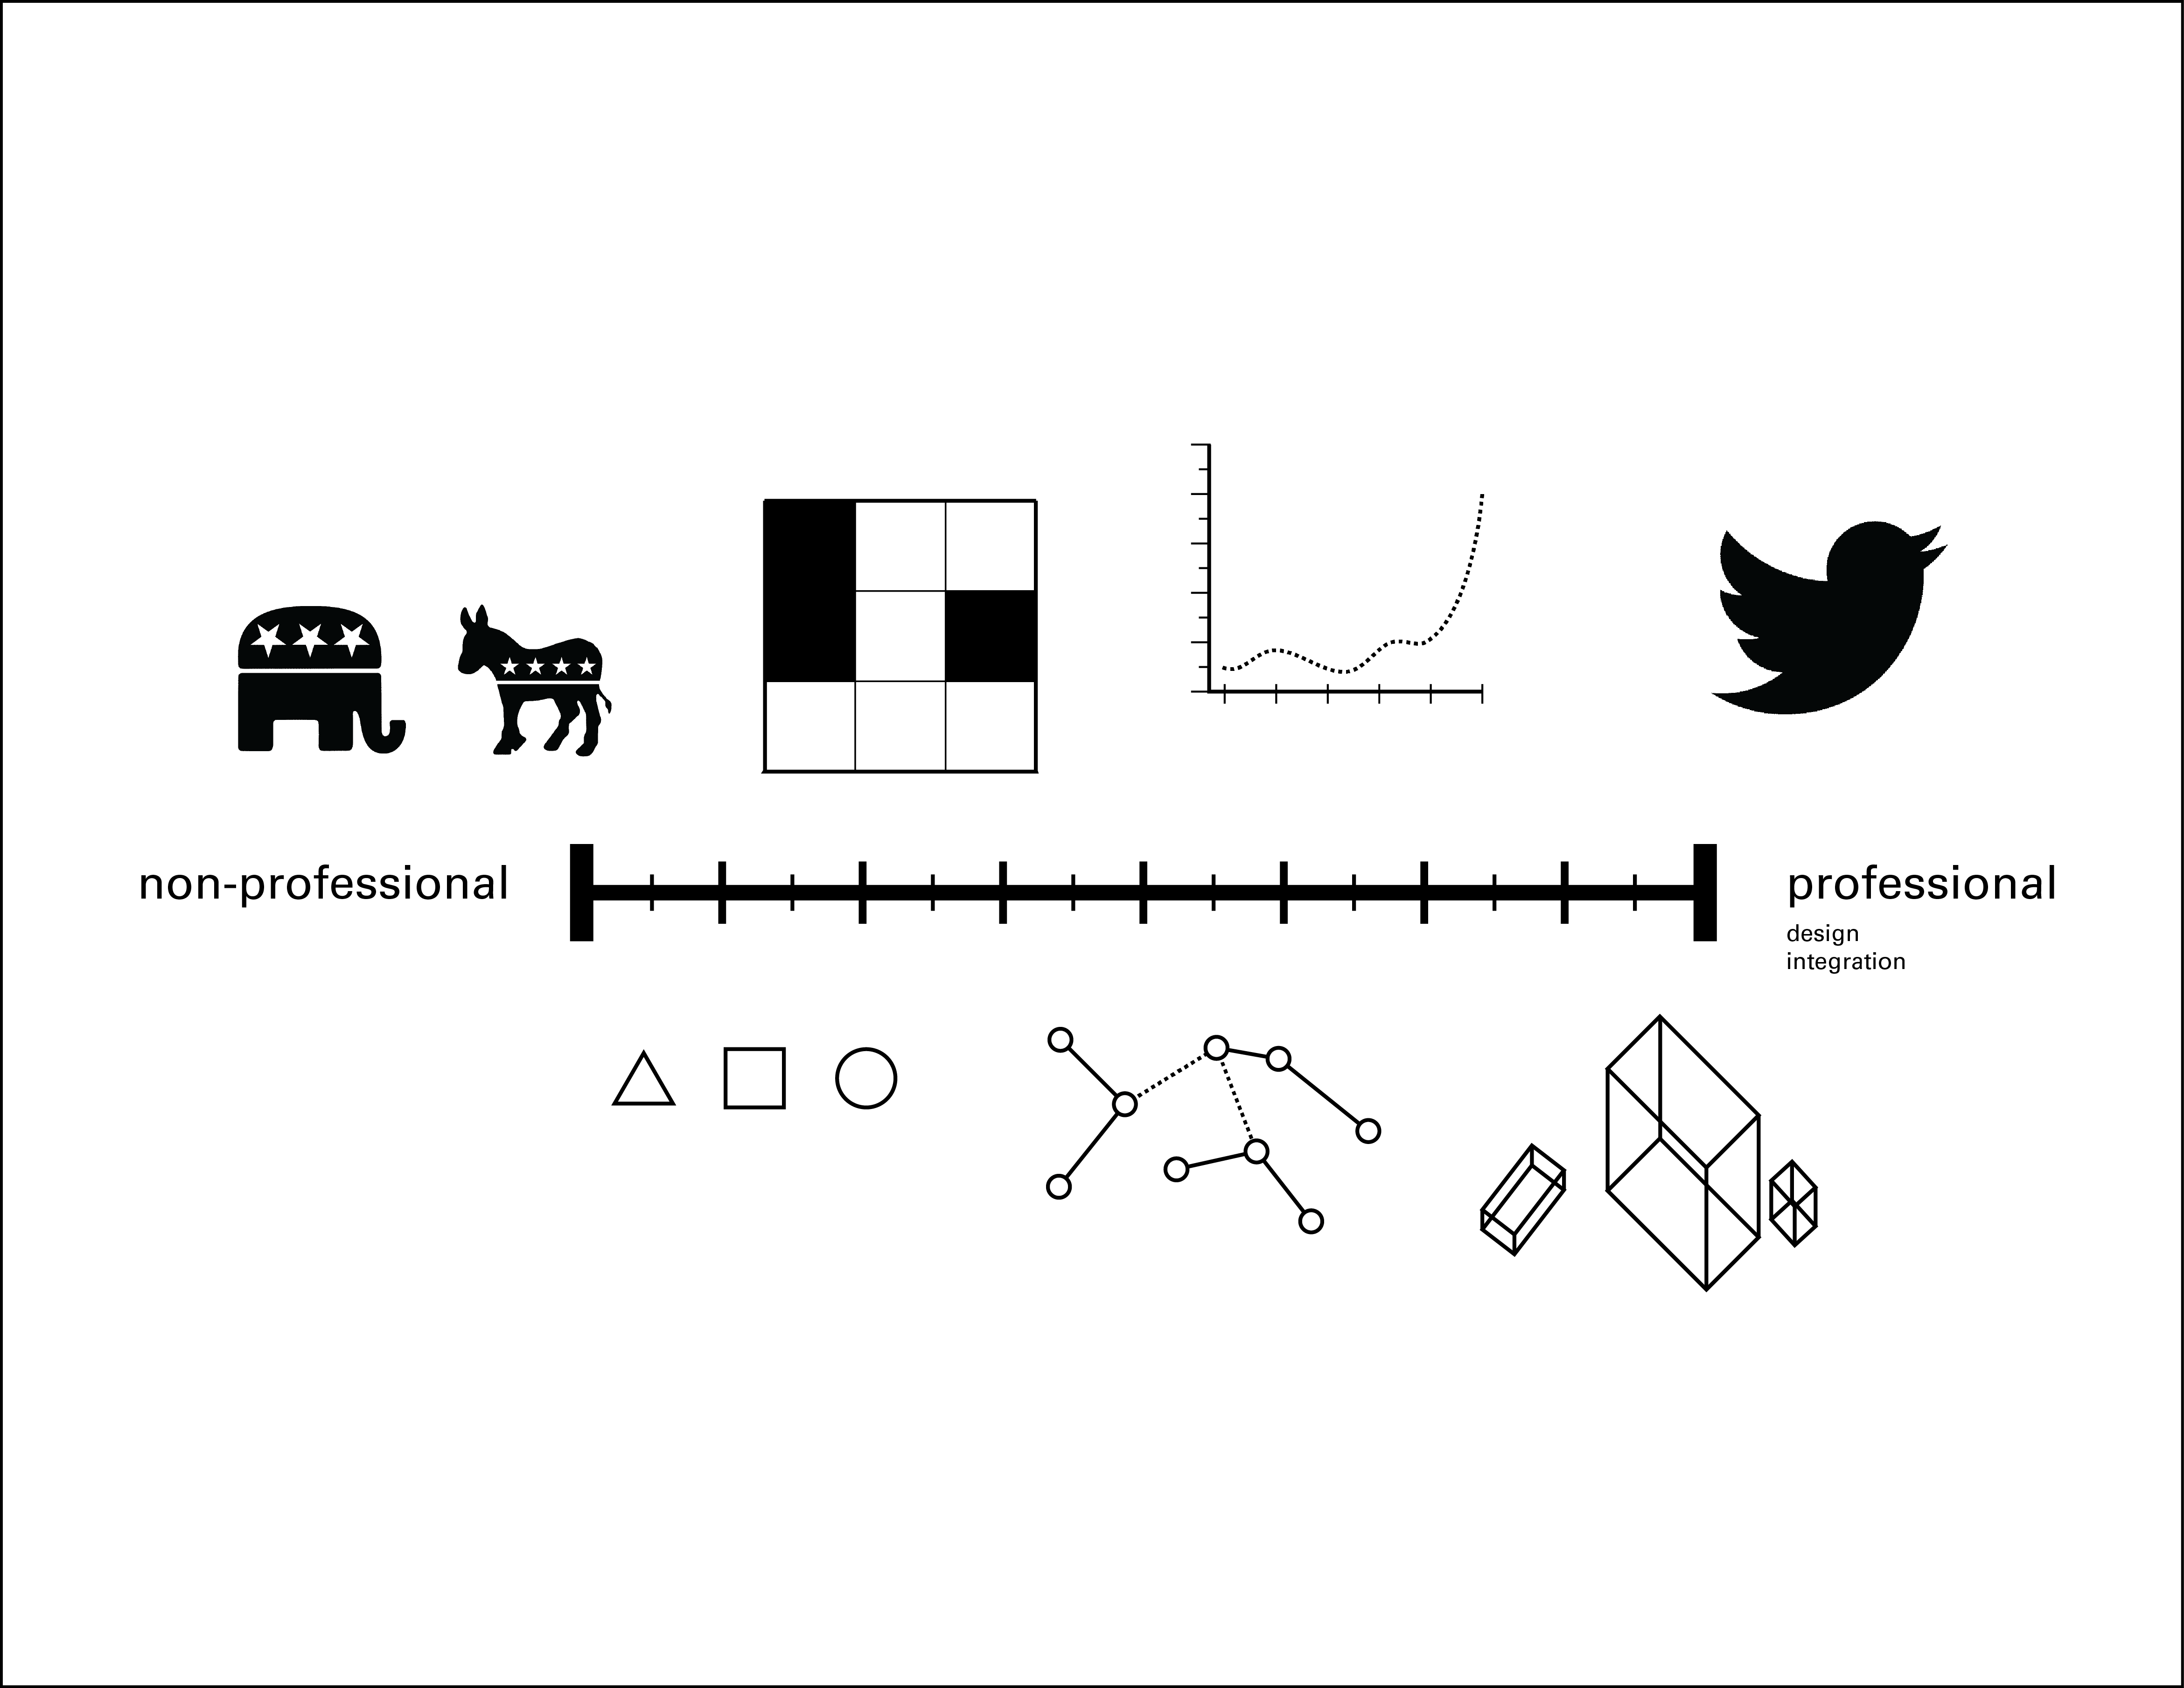
\includegraphics[width=\textwidth]{chapters/2/fig/spectrum.png}               
  \caption[number of bits per transaction]{Smaller the amount (bits) of
    information processed within one transaction, the easier to process. As it
    gets larger, it becomes unstructured data which is hard to directly convert
  to a decision or a intervention.}
  \label{fig:spectrum}
\end{figure}

The other side of the spectrum has richest information and can be seen in
an organized events to gather people in one place which include workshops,
focus groups,\dots etc. 
Although these events are organized and centralized to make it effective
for the head of the pyramid to listen, events are open ended, vocal and
unstructured which is hard to know the influence to the proposals the city
made. In any case the this information can be exchanged between
participants, and it is influenced by what kind of media is used for this
method.

\begin{marginfigure}[{15cm}]
  
\includegraphics[width=\textwidth]{chapters/1/fig/hearings.png}               
  \repeatcaption{fig:hearings}{Urban planners started different methods of "hearings" to centralize input from the community. Appendix \ref{app:traditional} shows different traditional methods}
\end{marginfigure}

\begin{figure}[htb]
  
\includegraphics[width=\textwidth]{chapters/2/fig/unstructured_app.png}               
  \caption[diagram: unstructured app]{
    Modern technology enables the community to provide data in a centralized way through collaborative data
    collection and analysis. Compared to the methods that do not leverage the
    media technology, these are better at collecting more data at once, since
  there is no physical constraints for gathering.}
  \label{fig:unstructured_app}
\end{figure}

Different types of media technology influence these methods of hearing. Talking to each other is the least constrained, which again is unstructured but rich.
% TODO:incomplete

\section{Professionals and citizens}

\begin{figure}[!htb]
  
\includegraphics[width=\textwidth]{chapters/2/fig/internalized_plan.png}               
  \caption[diagram: unstructured app]{Despite the innovation in "hearing" methods, this state still has the plan internalized in the top section of the pyramid.}
  \label{fig:internalized_plan}
\end{figure}

% TODO: strength the link between the diagram and paper

Until this point, the ``plan'' or the process of planning is still internalized inside the top sector. Yet there are reasons this project is receiving pressure to be externalized from both the community and the planners.

\subsection{the planning side and the ``wicked
problem''}\label{subsec:wicked}

The difficulty and complexity of social planning was addressed by Churchman
which coined the term ``wicked problems'' \cite{churchman1967guest}.
Churchman first points there are `tame' problems, which the issues are well
defined and is clear whether the problem was solved or not. Wicked problems
are the opposite which cannot be framed in a template and hard to
validate whether the problem is solved.
We can see the social planners depression by Churchman writing 
\begin{quotation}
  The lay customers are complaining because planners and other professionals have not
  succeeded in solving the problems they claimed they could solve.
\end{quotation}
According to Churchman, there are ten characteristics of a `wicked
problem', and one of them ``The social planner has no right to be wrong''
to ack politically.

Similar to the contrast of `tame' and `wicked' problems, other fields of
science also questioned the performance difference of professionals solve
problems compared to people that are non professionals. 
Johnson states this by the cognitive science and artificial
intelligence showing results that experts perform better compared to
novices while the empirical research in behavioral decision claims the
opposite. \cite{chi2014nature}
He continues that artificial intelligence focuses on structured
problems like chess, where the behavioral science looks into issues that
are hard to define the aspects and detangle the influences of each of them
such as predicting the market. As a result, have created a discrepancy of
the evaluation in the performance of experts.

% TODO: change 'hearings' to 'community meetings'
\begin{figure}[htb]
  
\includegraphics[width=\textwidth]{chapters/2/fig/externalized_plan.png}               
  \caption[diagram: externalized plan]{The plan has been externalized to the public. We see this by the current planning schema required to have a public meeting. (Although the strength of influence varies place to place.)}
  \label{fig:externalized_plan}
\end{figure}

Planners not being able to meet public demands, and not worthy of
predicting what is next, the gap between the public will increase.
Especially in current alternative media\footnote{Every thing other than
mainstream mass media.} tend to provide on what the general want to know
rather the what is true, making it increasingly difficult to correct.
This again aligns to Churchman's point in 1957 ``solutions to wicked problems are
not true or false, but good or bad.''

One possible method to overcome "wicked problems" is to take
a collaborative approach. \cite{roberts2000wicked}
\footnote{ The study examines three approaches, and concludes that the
  collaborative strategy is mode effective.
  \begin{itemize}
    \item Authoritative Strategies
    \item Competitive Strategies
    \item Collaborative Strategies
  \end{itemize}
}

Yet skills of collaboration are limited, especially among people who work
in a traditional bureaucracy with a strong hierarchy that limits
participation and team-based approaches to problem solving and decision
making.

New tools and methods are needed to support collaboration, inform people with different
perspectives, lower the cost of transaction, and provide a learning
experience on each topic, which is how we democratize the process
effectively

\subsection{Democratization}

There is evidence that urbanization triggers democratic
change\cite{woolley2010evidence} and urbanization is seen globally, 
we can assume the demand of democratization is in general increase.
John Dewey, who advocated on giving the community to collectively govern
themselves has pointed information and education are the key factors to
have the community undergo decision making.\cite{dewey2012public} 

Dewey emphasizes that the `new journalist' has two central roles; 1.verify
which information is reliable and 2.order it so the people can grasp it
efficiently.\footnote{ In a modern world, a system may be able to
do both using collective input.}
Shirky has pointed out that historically the balance between media
consumption and creation from the community was dominated by consumption,
but the advent of modern communication tools and the amount of output show
people also have the desire to create and share\cite{shirky2008here}.

% TODO: incomplete

The challenge is to transform individual experiences, frameworks and
perspectives into a shared, understandable, and, most importantly, a
transmittable area of knowledge.

\begin{figure}[htb]
  
\includegraphics[width=\textwidth]{chapters/2/fig/community_engagment.png}               
  \caption[diagram: community engagment]{Community engagement that will directly influence the plan}
  \label{fig:externalized_plan}
\end{figure}

People are now not only exposed the plan, but being able to provide
feedback. As of 2017, it is required by law to open a public meeting in
order to attain permit.

The level of participation is increasing, were people are now able to
communicate bi-directionally.
In the context of present planning procedures, this is pointed as community engagement.

\subsection{Extending Collective Intelligence}

Artificial intelligence has been gaining attention because of these
technologies advanced by the increase of available data as training sets.
The primary source of data is input from humans which as a group form a
collective intelligence. Extended Intelligence is a concept to apprehend
that intelligence was always a network and should incorporate both
artificial intelligence and collective intelligence to utilized them
mutually.\cite{pubpub:extended}
Hidalgo points out that network intelligence existed from the beginning and
cities are `` pockets where our species accumulates the capacity to produce
information''.\cite{hidalgo2015information} He mentions that the novelty
is today's technological context where computational resources have been
distributed more than ever before.\cite{pubpub:whatsnew}
Research says that the combination of these two types of
intelligence has potential to overcome the
performance\cite{baharad2011distilling}
in fields that were thought to have a little or no difference comparing
professionals and nonprofessionals. (p\pageref{subsec:wicked})

\subsection{Analysis and Synthesis}

In ``Notes on the Synthesis of Form'', Christopher Alexander, clearly
distinguishes that in a design procedure, there is always the analysis
phase before the synthesis phase and two are different.

\begin{quotation}
  Finding the right design program for a given problem is the first phase
  of the design process. It is, if we like, the analytical phase of the
  process. The first phase of the process must of course followed by the
  synthetic phase, in which a form is derived from the program. We shall
  call this synthetic phase the realization of the program.\cite{alexander1964notes}
\end{quotation}

There are few attempt that distinguishes these two process. Having the
premises that these two are different, there are fewer attempts to integrate
them in to the same platform. Figure\ref{fig:collective_design} shows one
example of such platform. 

\begin{figure}[htb]
  
\includegraphics[width=\textwidth]{chapters/2/fig/bikebump.png}               
  \caption[diagram: integrated collective design]{integrated design method
  that combines analytical and synthetic phase.}
\label{fig:collective_design}
\end{figure}

% The two parts of design is not clear in urban planning, only because the
% planner, or the top of the pyramid has always been the one who synthesizes.
% Where modern visualization can give insight outside the top part, the
% citizens have not found ways to do the analytical part. Now knowing the two
% parts, we can categorize the current tools whether it is for analysis or synthesis. 

